%%%%%%%%%%%%%%%%%%%%%%%%%%%%%%%%%%%%%%%%%%%%%%%%%%%%%%%%%%%%%%%%%%%%%%%
\documentclass[num-refs]{wiley-article} % Courtesy Overleaf

% Add additional packages here if required
\usepackage[numbers]{natbib}
\usepackage{natmove}
\usepackage{setspace}

%\changefontsizes{10pt}
\raggedbottom


% Update article type if known
\papertype{Original Article}
\paperfield{}

%\abbrevs{%
%         ABC, a black cat;
%	     DEF, doesn't ever fret;
%	     GHI, goes home immediately.
%     }

\title{Estimation for iron contamination in Si solar cell by ideality factor: deep neural network approach}

\author[1]{Oleg~Olikh}
\author[1]{Oleg~Lozitsky}
\author[1]{Oleksii~Zavhorodnii}

%\author[1\authfn{1}]{Oleg~Olikh}
%\author[1\authfn{1}]{Oleg~Lozitsky}
%\author[1\authfn{2}]{Oleksii~Zavhorodnii}


%\contrib[\authfn{1}]{Equally contributing authors.}

\affil[1]{Taras Shevchenko National University of Kyiv, 64/13, Volodymyrska Street, Kyiv, 01601, Ukraine}
%\affil[2]{Department, Institution, City, State or Province, Postal Code, Country}

\corraddress{Olikh O, Taras Shevchenko National University of Kyiv, 64/13, Volodymyrska Street, Kyiv, 01601, Ukraine}
\corremail{olegolikh@knu.ua}

%\presentadd[\authfn{2}]{Department, Institution, City, State or Province, Postal Code, Country}

\fundinginfo{National Research Foundation  of Ukraine, Project Number: 2020.02/0036}

%\runningauthor{F. Author et al.}

\begin{document}



Dear editor,

We like to express our appreciation to the reviewers for their comments.
We are resubmitting the revised version of the paper number PIP--21--281.
We have studied the comments of the reviewer carefully,
and have changed the text according to the comments they
have listed.
%The location of revisions is pointed by blue color in ``MarkedManuscript.pdf''.
Below we refer to each of the reviewer’s comments.


\subsection*{Response to Reviewer \#1 }



\noindent
\textcolor[rgb]{0.00,0.50,1.00}{\textbf{Comment~1.}}
\emph{A solar cell with BSF is chosen as the basis of the work, claiming that
"BSF is one of the popular designs used for industrial mass production...",
but this is no longer the case, BSF solar cells are present in the market due to old manufacturing lines that are still operative, but the standard now is PERC technology.
If the training of the network is based on SCAPS simulations, why was not trained with a PERC structure?
At least, some hint on how results would be with a PERC structure should be given.
(By the way, the BSF in this work is made with B-doping, which is also a minoritary approach at the industrial level, where BSF is of Aluminium).}

\vspace{0.5cm}
\noindent
\textcolor[rgb]{0.51,0.00,0.00}{\textbf{Reply:}}
The Reviewer is absolutely right that PERC technology will be dominant in near future.
But now the part of BSF solar cells is still big enough --- see Fig.~\ref{fig_BSF}.


\begin{figure}[b]
\centering
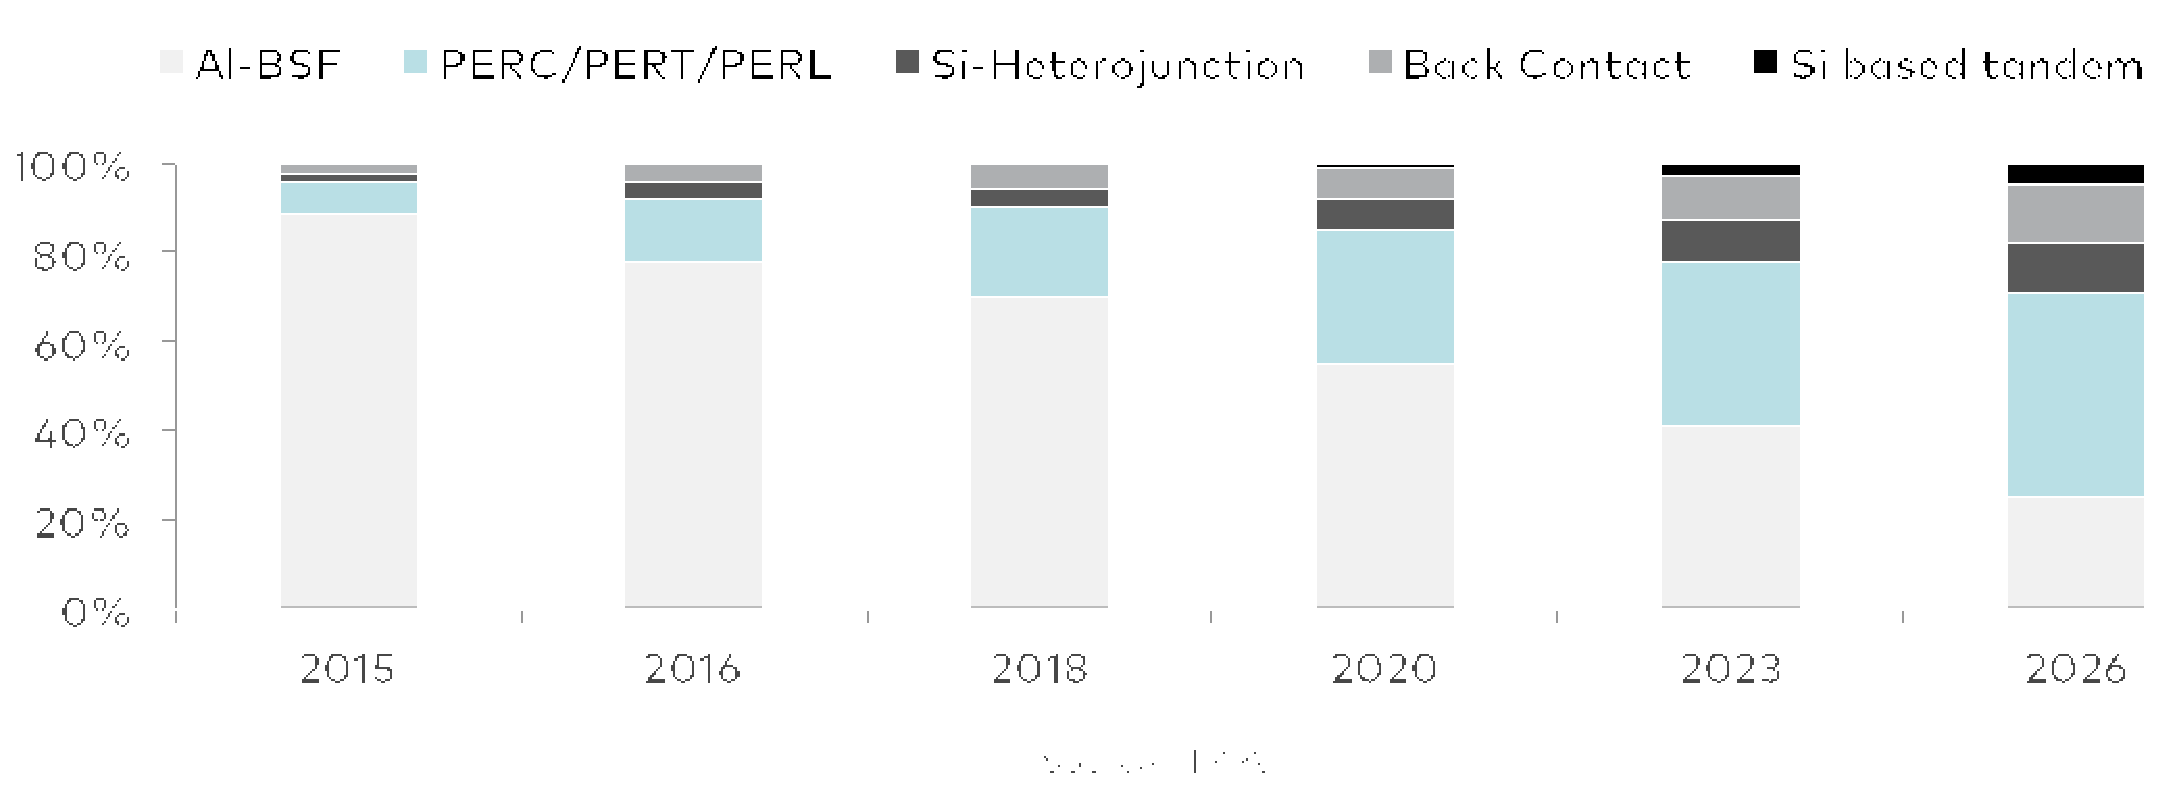
\includegraphics[width=0.48\textwidth]{BSF_PERC1}
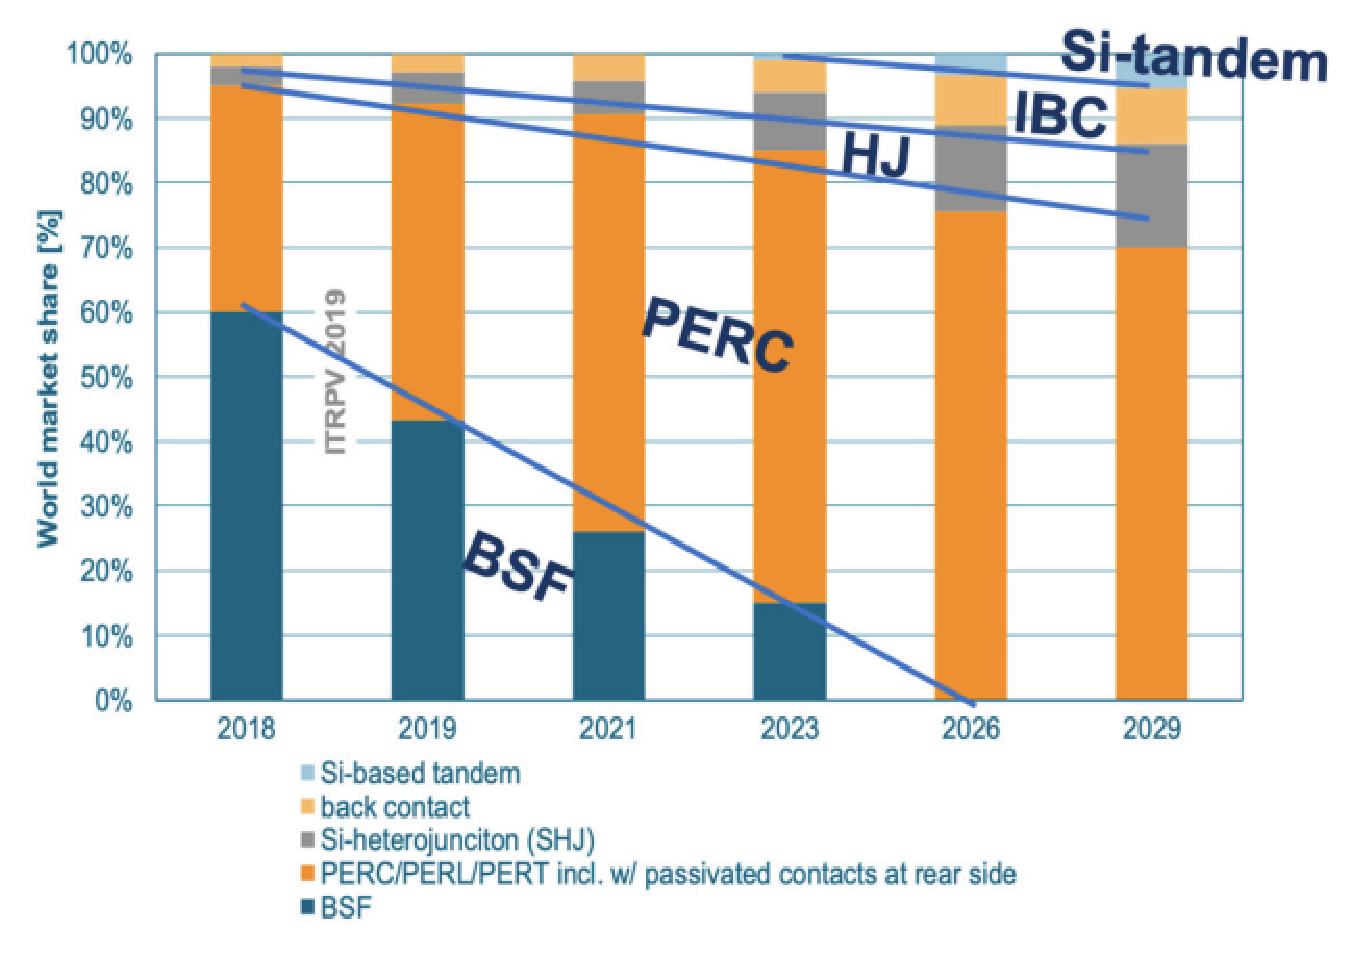
\includegraphics[width=0.48\textwidth]{BSF_PERC2}
\caption{Projected manufacturing capacity share of different
silicon--based cell technologies.
Sources:  https://www.aleo-solar.com/perc-cell-technology-explained/
(left panel), \cite{GreenRew2019} (right panel).
}
\label{fig_BSF}
\end{figure}

SCAPS-1D is a one-dimensional solar cell simulation program, so to model PERC solar cells with a rear contact,
which is inhomogeneous in a surface, is a rather hard job.
We understand the restrictions of 1D simulators and point out this fact in the Conclusion.

We agree that it would be better to use an Al-doped $p^+$-layer, but our choice was determined by the following considerations.
The simulated IV curves were used to obtain the ideality factor $n$.
According to the two-diode model we applied,
$n$ characterizes the current of the second (or so-called recombination) diode
which arises due to recombination occurring mainly within the depletion region \citep{Breitenstein2013,n2McIntosh}.
The probable $p^+$--layer influences this process mostly via the electric field.
Therefore, the kind of doping atom in the $p^+$--layer is not very important for our simulation.
In the case of $n^+-p-p^+$ structure with Al-doped base,
a new dataset will be certainly required for training DNN.
However, the deep-learning oriented approach for determining impurity concentration that we propose remains quite applicable.
Besides, the recombination in the rear surface region is not crucially important for estimating the ideality factor.
In our opinion, the trained DNNs can be applied to PERC solar cell in which
i)~the base is boron-doped;
ii)~the iron-related deep levels are the main cause of defect-assisted recombination.

The text was revised and some speculations about applicability of the trained DNNs were added (last three paragraph before Conclusion).

\vspace{1cm}
\noindent
\textcolor[rgb]{0.00,0.50,1.00}{\textbf{Comment~2.}}
\emph{As far as I understand, the simulation with SCAPS could be improved: emitter and BSF are uniform and this is not the case in reality.
There is no mention to the metallization, are there no contacts?
There should be, and they will influence the carrier transport and also the surface recombination velocities in the metal-semiconductor interface, among others.}

\vspace{0.5cm}
\noindent
\textcolor[rgb]{0.51,0.00,0.00}{\textbf{Reply:}}
For metal contacts on the rear and front surfaces,
the flat bands' conditions were assumed.
The appropriate sentence was added to the text.
It should be noted that it is a common practice in SCAPS simulation not to pay much attention to contacts
in case they do not create additional barriers --- e.g., see \cite{SCAPSuseSi4,SCAPSuseSi1,SCAPSuse1,SCAPSuse5,ScapsUse10}.


We share the Reviewer’s view on the way of improving SCAPS simulation.
In the present paper, we concentrate on recombination in the SC base region,
which mainly determines the ideality factor.
As for the non-uniformities of emitter and  BSF-layer, their effect on $n$ is much weaker.
In any case, the Reviewer’s suggestion is very valuable, and we are going to consider it in the future.

\begin{figure}[t]
\centering
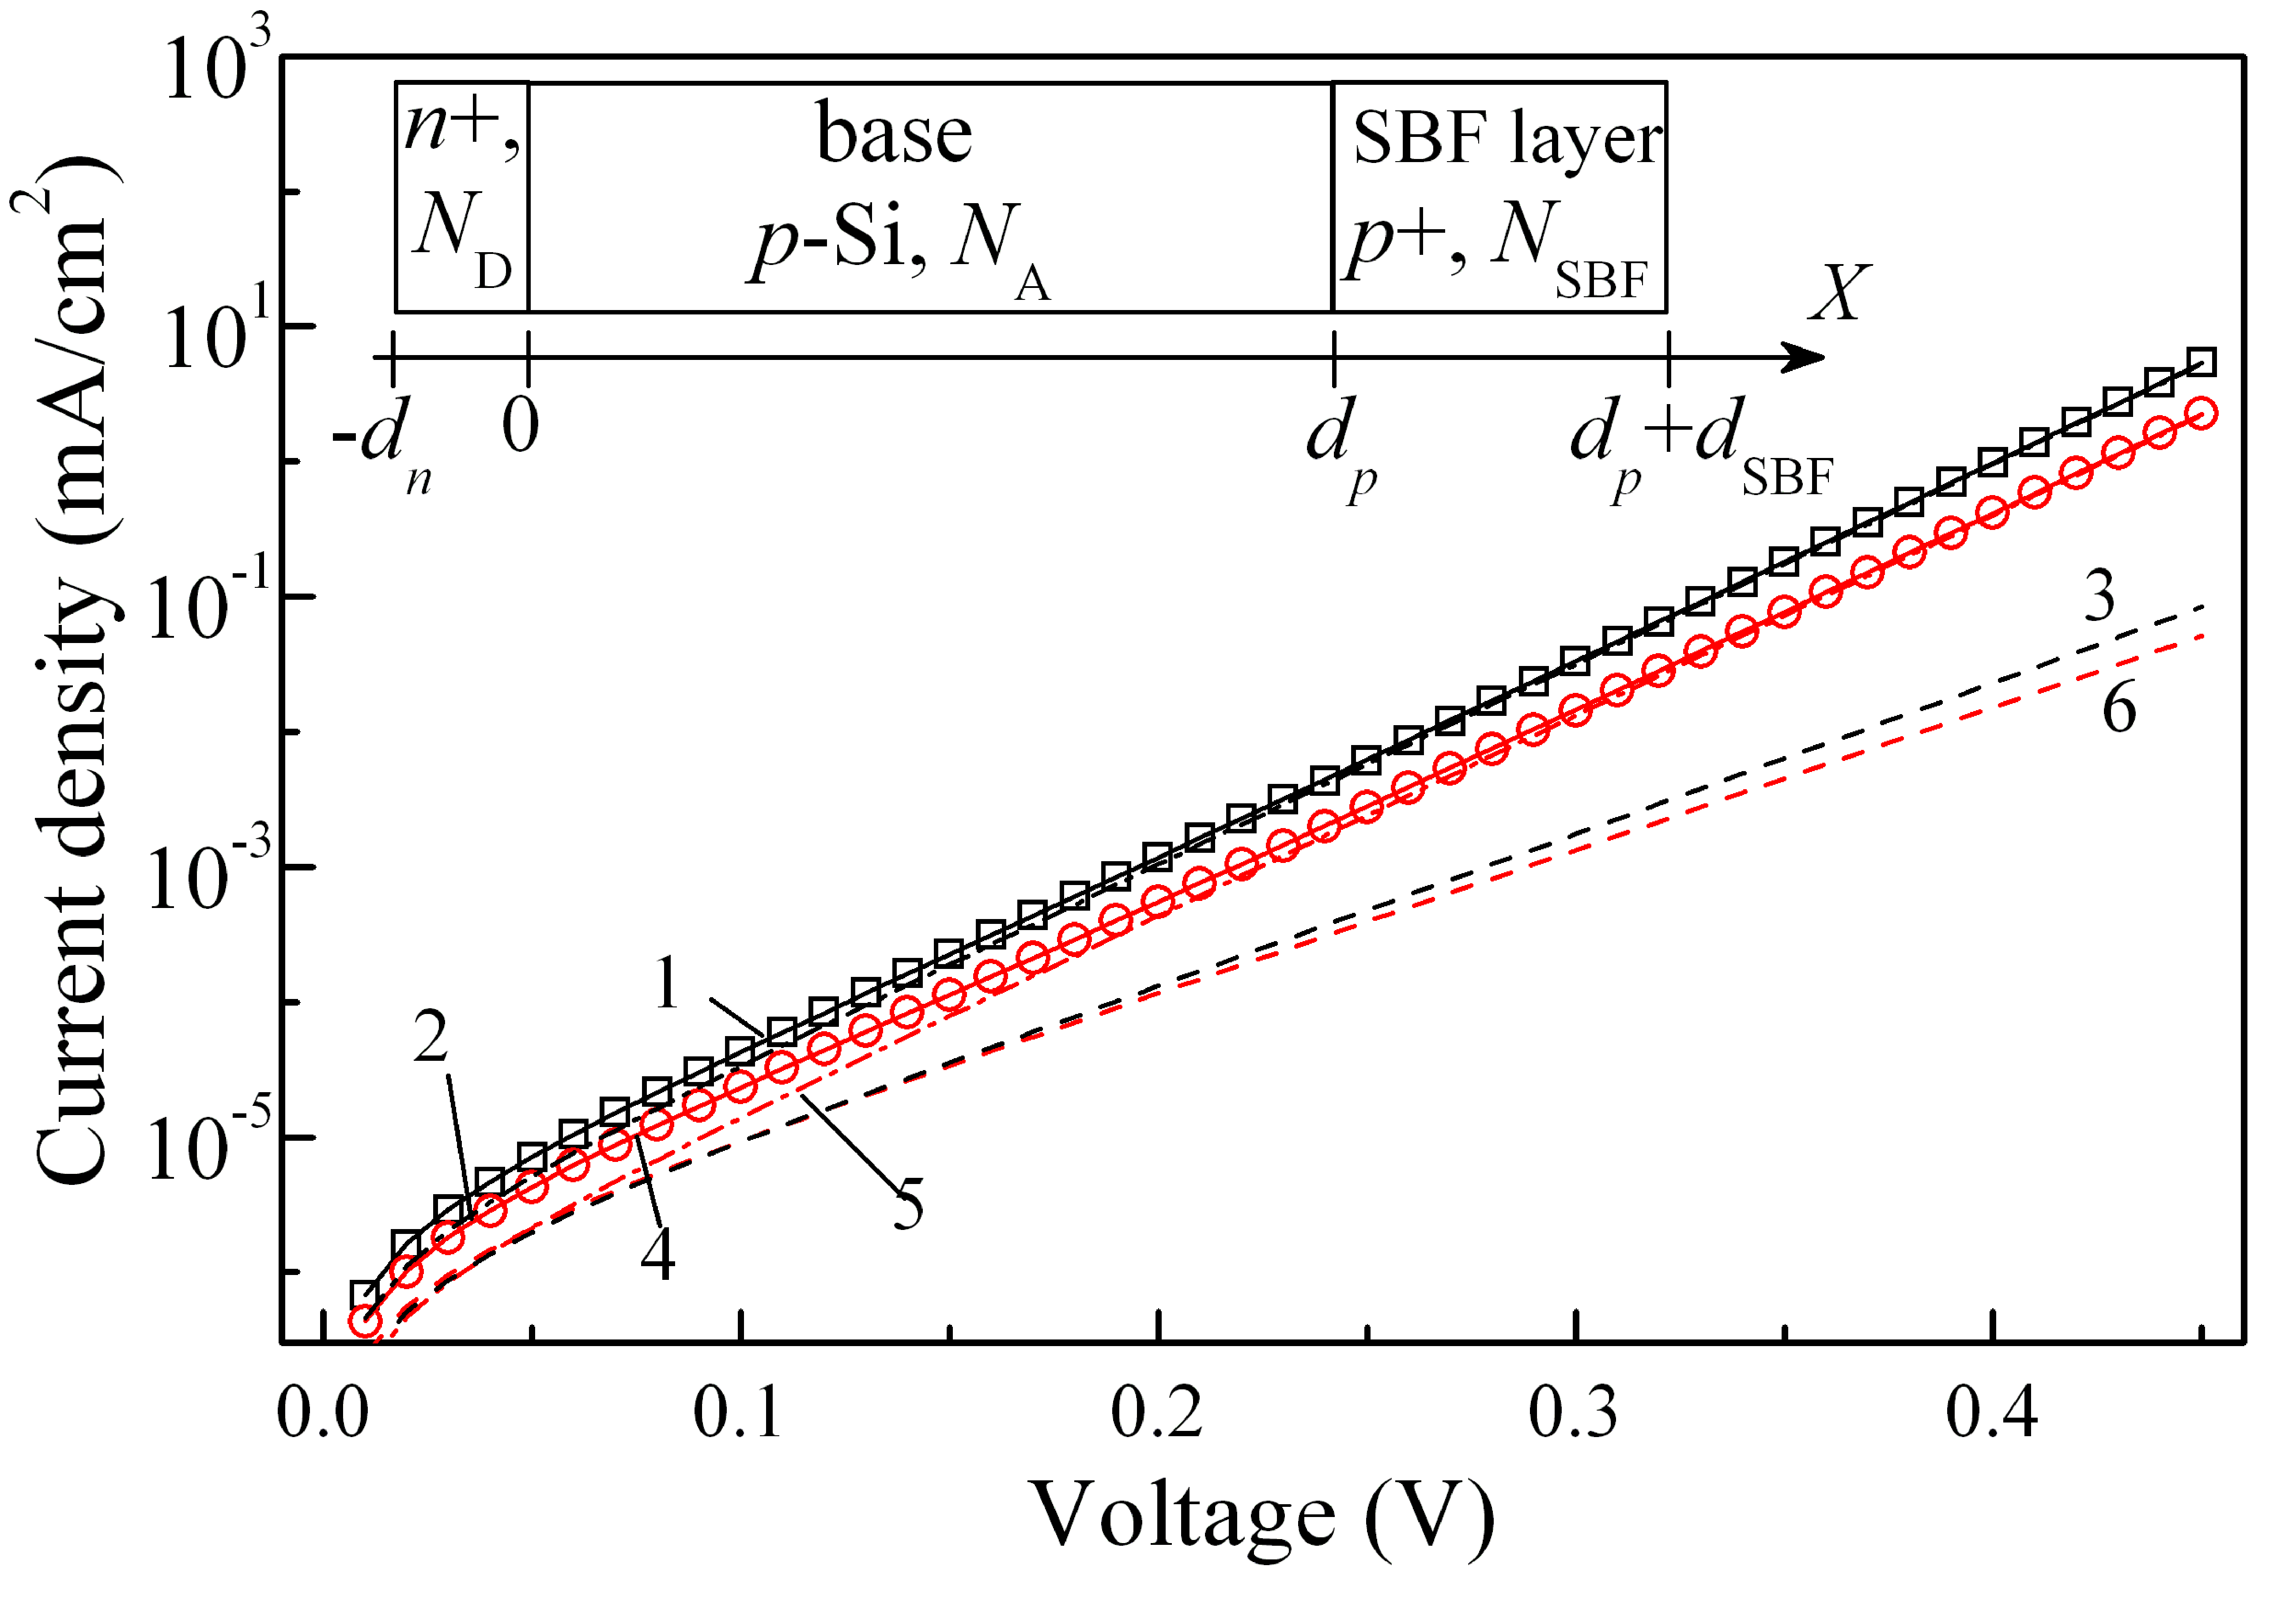
\includegraphics[width=0.5\textwidth]{FigIV}
\caption{Simulated IV characteristic (marks)
and its fitting by Eq.~(\ref{eqIVd}) (solid lines 1 and 4).
The dashed (3, 6) and dotted--dashed (2, 5)
lines represent the recombination diode currents and the ``ideal'' diode currents, respectively.
$N_\mathrm{B} = 10^{17}$~cm$^{-3}$, $N_\mathrm{Fe} = 10^{13}$~cm$^{-3}$,
$T = 340$~K, $d_p = 180$~$\mu$m.
The results for Fe-case (circles, curves 4-6, red)
and Fe-FeB case (squares, curves 1-3, black) are presented.
Inset: Structures, which are used in the simulation.
}
\label{fig_IV}
\end{figure}


\vspace{1cm}
\noindent
\textcolor[rgb]{0.00,0.50,1.00}{\textbf{Comment~3.}}
\emph{Why a voltage sweep restricted to 0.45 V?
This is rather low when compared to the voltages at the maximum power point of BSF solar cells...
Wouldn't it influence in the extraction of the ideality factor values?}

\vspace{0.5cm}
\noindent
\textcolor[rgb]{0.51,0.00,0.00}{\textbf{Reply:}}
In order to fit the simulated data the two-diode model was used,
according to which the dark SC current is given by
\begin{equation}
\label{eqIVd}
    I=I_{01}\left[\exp\left(-\frac{q(V-R_sI)}{kT}\right)-1\right]
      + I_{02}\left[\exp\left(-\frac{q(V-R_sI)}{nkT}\right)-1\right]
      +\frac{V-R_sI}{R_{sh}}\,,
\end{equation}
where
$I_{01}$ and $I_{02}$ are saturation currents,
$R_{sh}$ and $R_s$ are shunt and series resistances.
The two-diode model is often applied to describe real Si SCs:
in Eq.~(\ref{eqIVd}) the first diode represents the ``ideal'' diode
and the first term in the equation describes recombination
in the base depth and emitter, including their surfaces;
the second diode is the so-called recombination diode
and the second term describes recombination within the depletion region \citep{Breitenstein2013}.


Typical IV curves are shown in Fig.~\ref{fig_IV}.
It is seen that the contribution of recombination diode current is essential at low bias only.
At $V\simeq 0.25$~V the first term in Eq.~(\ref{eqIVd}) is
by an order of magnitude greater than the second one
(see difference between the dotted-dashed fitting line and dashed fitting line).
A similar situation is observed for
experimental IV curves --- see Fig.~9 in Manuscript.
The ideality factor correlates with  the slope of the recombination current
plotted against the voltage in a semi-logarithmic scale.
Therefore the voltage range $(0-0.45)$~V is quite sufficient for determining the ideality factor quite accurately.


The information was added on page 5, the first paragraph from the top;
the typical IV curves was added in Supplementary Material.


\vspace{1cm}
\noindent
\textcolor[rgb]{0.00,0.50,1.00}{\textbf{Comment~4.}}
\emph{I am not sure that I interpret well the results in table 5.
In the text the authors state that "the results even exceed expectations".
But what I see is that the predictions fail in general, largely for the trained dataset cases,
but also for the full dataset.
There is some discussion on why DNN$_{FeFeB-Fe}$ performs worse than DNN$_{FeFeB}$
and that is Ok... but DNN$_{FeFeB}$ also fails in many cases, isn't it?
(temperatures higher than 300K for the higher Fe content,
100\% or more error for the training dataset...).
}

\vspace{0.5cm}
\noindent
\textcolor[rgb]{0.51,0.00,0.00}{\textbf{Reply:}}
On the one hand, the Reviewer is right.
Unfortunately, DNNs  trained by synthetic data
proved incapable of measuring iron concentration
with high precision in real solar cells
(with a certain mismatch between real parameters and those used in the simulation).
From this point of view the ``glass is half empty''.

On the other hand, there are also some reasons
to say that the ``glass is half full''.
First of all, in our opinion,
the low cost express method which uses a widely applied setup and is able
to estimate approximately the range of iron concentration
(even with 100\% error) can be quite useful.
At the same time there are possible ways to improve precision  and these are discussed in the Conclusion.
Moreover, the results in Table~5 prompt how this method can be appropriately used in practice.
First, the near room temperature of IV measurement is preferable
(this conclusion is similar to those drawn from the analysis of synthetic IVs);
second, the time between FeB pair dissociation and IV measurement must be as short as possible.
Finally, in some cases (300~K, ``full'' dataset) the DNN$_\mathrm{FeFeB}$ can yield acceptable results.


We hope that the  retrieval of deep level parameters
from the current--voltage curve by deep learning
will be further improved.


\vspace{1cm}
\noindent
\textcolor[rgb]{0.00,0.50,1.00}{\textbf{Comment~5.}}
\emph{In the jargon, we do not talk of surface resistance, but sheet resistance.
Also, it is the first time that I read the "anti-recombination isotype barrier" for a high-low junction or a BSF.}

\vspace{0.5cm}
\noindent
\textcolor[rgb]{0.51,0.00,0.00}{\textbf{Reply:}}
The Reviewer is absolutely right.
We have revised the text accordingly.

\vspace{1cm}
\noindent
\textcolor[rgb]{0.00,0.50,1.00}{\textbf{Comment~6.}}
\emph{It is mentioned in the paper that there is Suplementary Material, but I have not had the opportunity to read it.}

\vspace{0.5cm}
\noindent
\textcolor[rgb]{0.51,0.00,0.00}{\textbf{Reply:}}
We apologize for the embarrassment, but there must be some technical confusion:
Reviewer \#2 mentioned the data in the table of Supplementary Material.

\vspace{1cm}
\noindent
\textcolor[rgb]{0.00,0.50,1.00}{\textbf{Comment~7.}}
\emph{On the other hand, the paper needs a thorough revision of English, preferably by a native or bilingual speaker.
English is not my mother tongue, but I think that there are many expressions that are not correct, and make the reading difficult.
From the abstract ("The low-cost and express...", "an ideality factor values"...)
to the conclusions ("not numerous input parameters can be multiplied and transformed to the picture and apply a vision model..."(?),
and a lot in between: "both for microelectronics, logic technologies and solar cells",
"the various semiconductor barrier structures", "practical using", "Fours", "SFB", "in our further calculation",
"simulated with using", "in comparing with", "more narrow", etc. etc. }

\vspace{0.5cm}
\noindent
\textcolor[rgb]{0.51,0.00,0.00}{\textbf{Reply:}}
We are sorry for our English.
The text has been revised by a bilingual speaker, and we hope for the language improvement.


\subsection*{Response to Reviewer \#2 }


\textcolor[rgb]{0.00,0.50,1.00}{\textbf{Comment~1.}}
\emph{2 Simulation details}

\emph{It is assumed that all SRH recombination in the device come from iron impurities and the associated deep level defects.
It seems necessary to discuss its validity, and it could be interesting to put it against the fact that Al-BSF devices based on Czochralski silicon wafers are considered.
More generally, if another type of defects is present in the solar cell, also inducing SRH recombination,
is it possible to estimate to what extend are the DNNs trained here still accurate ? }

\vspace{0.5cm}
\noindent
\textcolor[rgb]{0.51,0.00,0.00}{\textbf{Reply:}}
The speculations about the applicability of the trained DNNs to different SC structures
must be based on assumption that the ideality factor distinguishes
depletion-region recombination from most other sources of recombination \cite{Breitenstein2013,n2McIntosh}.
Certainly, there are some deviations from this rule for real structures.
For instance, our simulation reveals the $n$ dependence on base thickness \cite{OlikhJPS}.
Nevertheless this dependence is weak, and the ideality factor value is mainly determined
by depletion-region recombination.



Also, the DNNs applicability depends on the requirement for Shockley–Read–Hall recombination to be predominant.
In case,
if there are other mechanisms causing free carrier concentration to decrease,
the models which diverge from the two-diode one are proposed
(e.g., three-diode \cite{TreeDiode,Shah}).
Moreover, the base must be doped by boron.
For example, if SC is prepared from Si:Al wafer,
the simulation model which is used for training dataset preparation must be modified:
the parameters of $\mathrm{Fe}_i\mathrm{Al}_s$ pair as well as
the changes in defect distribution (Eq.~(9)) should be taken into consideration.
Finally, if another type of defect (in addition to iron--related deep levels)
is present in the solar cell, which also induces intensive SRH recombination,
the simulation model must be more complicated as well.
The primary competitors of $\mathrm{Fe}_i\mathrm{B}_s$  are  boron-oxygen complexes \cite{LIDRev,LIDRev2}
and oxide precipitates \cite{MurphySC2014,Oxide:Chen} in Cz-Si.
So the development of the corresponding model can be our next step.
To the point, it should be noted that a high $n$ value can serve as an indicator of another defect presence:
in our simulation this value is $n<1.4$.
The absence of non-iron active defects may be the most limiting factor of the DNNs applicability;
in particular, this confined the selection of SCs for our experimental verification of the proposed method.

Thus, the trained DNNs can be applied to BSF solar cells prepared from Si:B wafers.
It should be noted that the modern  technique of crystal growth
makes it possible to restrict
oxygen concentration substantially even in solar grade Cz-Si.
On the one hand,  Al is used to produce the doped $p^+$ region
at the industrial level \cite{GreenRew2019,WilsonRew2020}.
However, boron BSF is one of the promising techniques
for achieving high quality back contact \cite{Kim2007,B-BSF}
and for this reason  the $p^{+}$ layer, which is doped by boron, was under our consideration.
On the other hand, the probable $p^+$--layer influence on the depletion-region recombination
process is determined mainly by the electric field.
Therefore, the kind of doping atom in $p^+$--layer is not very important for simulation,
and in our opinion, the  DNNs is applicable for Al BSF cell as well.

Our speculations concerning this issue were added to the Manuscript ( the last three paragraphs before Conclusion).

\vspace{1cm}
\noindent
\textcolor[rgb]{0.00,0.50,1.00}{\textbf{Comment~2.}}
\emph{When Fe-FeB and Fe cases are presented, it could be clearer to provide very few more explanations on both types of defects,
and the important fact that iron-boron pairs can be temporarily dissociated, providing the Fe case,
through the heat treatment or high illumination already mentioned. }

\vspace{0.5cm}
\noindent
\textcolor[rgb]{0.51,0.00,0.00}{\textbf{Reply:}}
The corresponding corrections were made on page 4, the third  paragraph from the top.


\vspace{1cm}
\noindent
\textcolor[rgb]{0.00,0.50,1.00}{\textbf{Comment~3.}}
\emph{3 Deep neural network models}

\emph{
It is clear how the main training dataset is created, and how the 4 * 9 * 11 * 19 = 7524 IV curves are generated.
However, the definition of the test datasets and the values for temperature,
base thickness, iron concentration and doping level are not clear for each T-varied, d-varied, etc. test set. }

\vspace{0.5cm}
\noindent
\textcolor[rgb]{0.51,0.00,0.00}{\textbf{Reply:}}
As an example, we added the parameter values used for creating Fe-varied dataset
in the last paragraph on page 5 and the first paragraph on page 6.

\vspace{1cm}
\noindent
\textcolor[rgb]{0.00,0.50,1.00}{\textbf{Comment~4.}}
\emph{
For instance, in the case of the T-varied test set, it is mentioned that the same base thickness,
iron concentration and doping level values are used as in training dataset.
However, 4 * 9 * 19 = 684 and the amount of 894 IVs can’t be explained by multiplying with any number of temperature values.
In Supplementary Material, the associated summary table do neither explain this value 894. More generally these tables are difficult to interpret. It is possible that the subset of 144 values for T-varied test has been duplicated. }

\vspace{0.5cm}
\noindent
\textcolor[rgb]{0.51,0.00,0.00}{\textbf{Reply:}}
The Reviewer is  right:
i)~the subset of 144 values for the T-varied test dataset has been duplicated;
ii)~Table in Supplementary Material has mistakes and is not clear.
The correct values of $d_p$, $N_\mathrm{B}$, $T$, and $N_{\mathrm{Fe}}$ were listed in Table,
but there were problems with addition and multiplication
and we apologize for being inattentive.
The Table in Supplementary Material has been revised.


\vspace{1cm}
\noindent
\textcolor[rgb]{0.00,0.50,1.00}{\textbf{Comment~5.}}
\emph{4 Results and discussion}

\emph{
On figures 4, 5, 6 and 7, very interesting results are presented,
and analyses of the dependence of estimation
error with temperature, boron or iron densities and base thickness are well done.
However, it seems that the same error statistics of results obtained on test datasets
(instead of training dataset) would more directly assess the quality of predictions by the DNNs.
For instance, the Fe-varied dataset has been identified to be
the closest to “real demand” or results obtained with the all-varied dataset
would also be most probably very useful.
Such results could be showed in Supplementary Material, in the same form as figures 4, 5, 6 and 7. }

\vspace{0.5cm}
\noindent
\textcolor[rgb]{0.51,0.00,0.00}{\textbf{Reply:}}
The Supplementary Material has been completed by the figures
that  represent similar results for test datasets (Figs.~8S--11S).

However, it should be noted that error statistics for the training dataset is more correct and informative.
For instance, let us consider the temperature dependence (Fig.~4(a)).
In fact, averaging over 684 values was performed for each of 11 points in the training dataset,
and in fact these values correspond to the data uniformly distributed over used $(N_\mathrm{Fe},N_\mathrm{B},d_p)$-space.

In contrast, only 55 IV characteristics correspond to $T=295$~K in the Fe-varied dataset
(see Table in Supplementary Material).
In the All-varied dataset,
the six  temperature values that have been used are in the range $290-315$~K and only three values are in the range  $315-340$~K.
Moreover, eight IV characteristics were simulated at $T=293$~K for $N_\mathrm{Fe}=(5-9)\times10^{12}$~cm$^{-3}$
(high values)
whereas 60 ideality factor values are available at $T=292$~K,
with $N_\mathrm{Fe}=1.1\times10^{10}-5\times10^{12}$~cm$^{-3}$ being used to simulate corresponding IV curves.
So, it does not seem quite correct to compare data at  $T=292$~K with data at $T=293$~K.




%\bibliographystyle{rss}
\bibliographystyle{WileyNJD-Harvard}
\bibliography{olikh}


\end{document}
